\section{Data Description}
Standartox constitutes a collection of 600,000 quality checked ecotoxicological test results comprising roughly 8000 distinct chemicals and 8000 taxa that allows for the retrieval of single toxicity equivalents. It is build on the ECOTOX database \citep{usepa_ecotox_2019} and the data are processed to clean and harmonise entries to retrieve comparable toxicity endpoints. Subsequently, filter and aggregation methods are provided to allow for the retrieval of single toxicity equivalents for specific experimental conditions. The underlying ECOTOX database is updated quarterly and provides on average 5228 (2014 - 2019) new toxicity entries with each update. As soon as a new update of ECOTOX is available, Standartox is directly built in an automated way and therefore incorporates new data steadily. Standartox comes with a version control to guarantee reproducibility, meaning that once derived Standartox estimates can be retraced at a later stage, although new data might have updated the estimates already. Users can reach Standartox via a web application and an R-package (standartox) that accesses an application programming interface (API) providing the possibility of scriptable requests.

\subsection{Filters}
The data can be restricted to the three endpoint groups, namely half maximal effective/lethal concentration/dose values (e.g. EC50, LD50), henceforth abbreviated as XX50, lowest observed effect levels/concentrations (LOEC/L), henceforth abbreviated as LOEX and no observed effect levels/concentrations (NOEL/C), henceforth abbreviated as NOEX (Table \ref{tab:endpoints-conflate}). Standartox allows the ecotoxicity data to be filtered by 23 distinct effect groups (e.g. mortality, population, growth) (Fig. \ref{fig:stx-parameters}B) and concentration types (e.g. formulation, active ingredient). In addition to these test-specific parameters, Standartox data entries can be filtered by chemical-specific parameters such as the CAS number and chemical classes (e.g. pesticides, metals, drugs) (Fig. \ref{fig:stx-parameters}C). Furthermore, the Standartox data can be refined to organism-specific parameters, such as the organism habitat (e.g. freshwater, marine, terrestrial) (Fig. \ref{fig:stx-parameters}E), their occurrence regions (e.g. Europe, South America) (Fig. \ref{fig:stx-parameters}F) as well as different taxonomic levels. Additionally users can refine the results to specific test durations (in hours).

\begin{figure}[h!]
    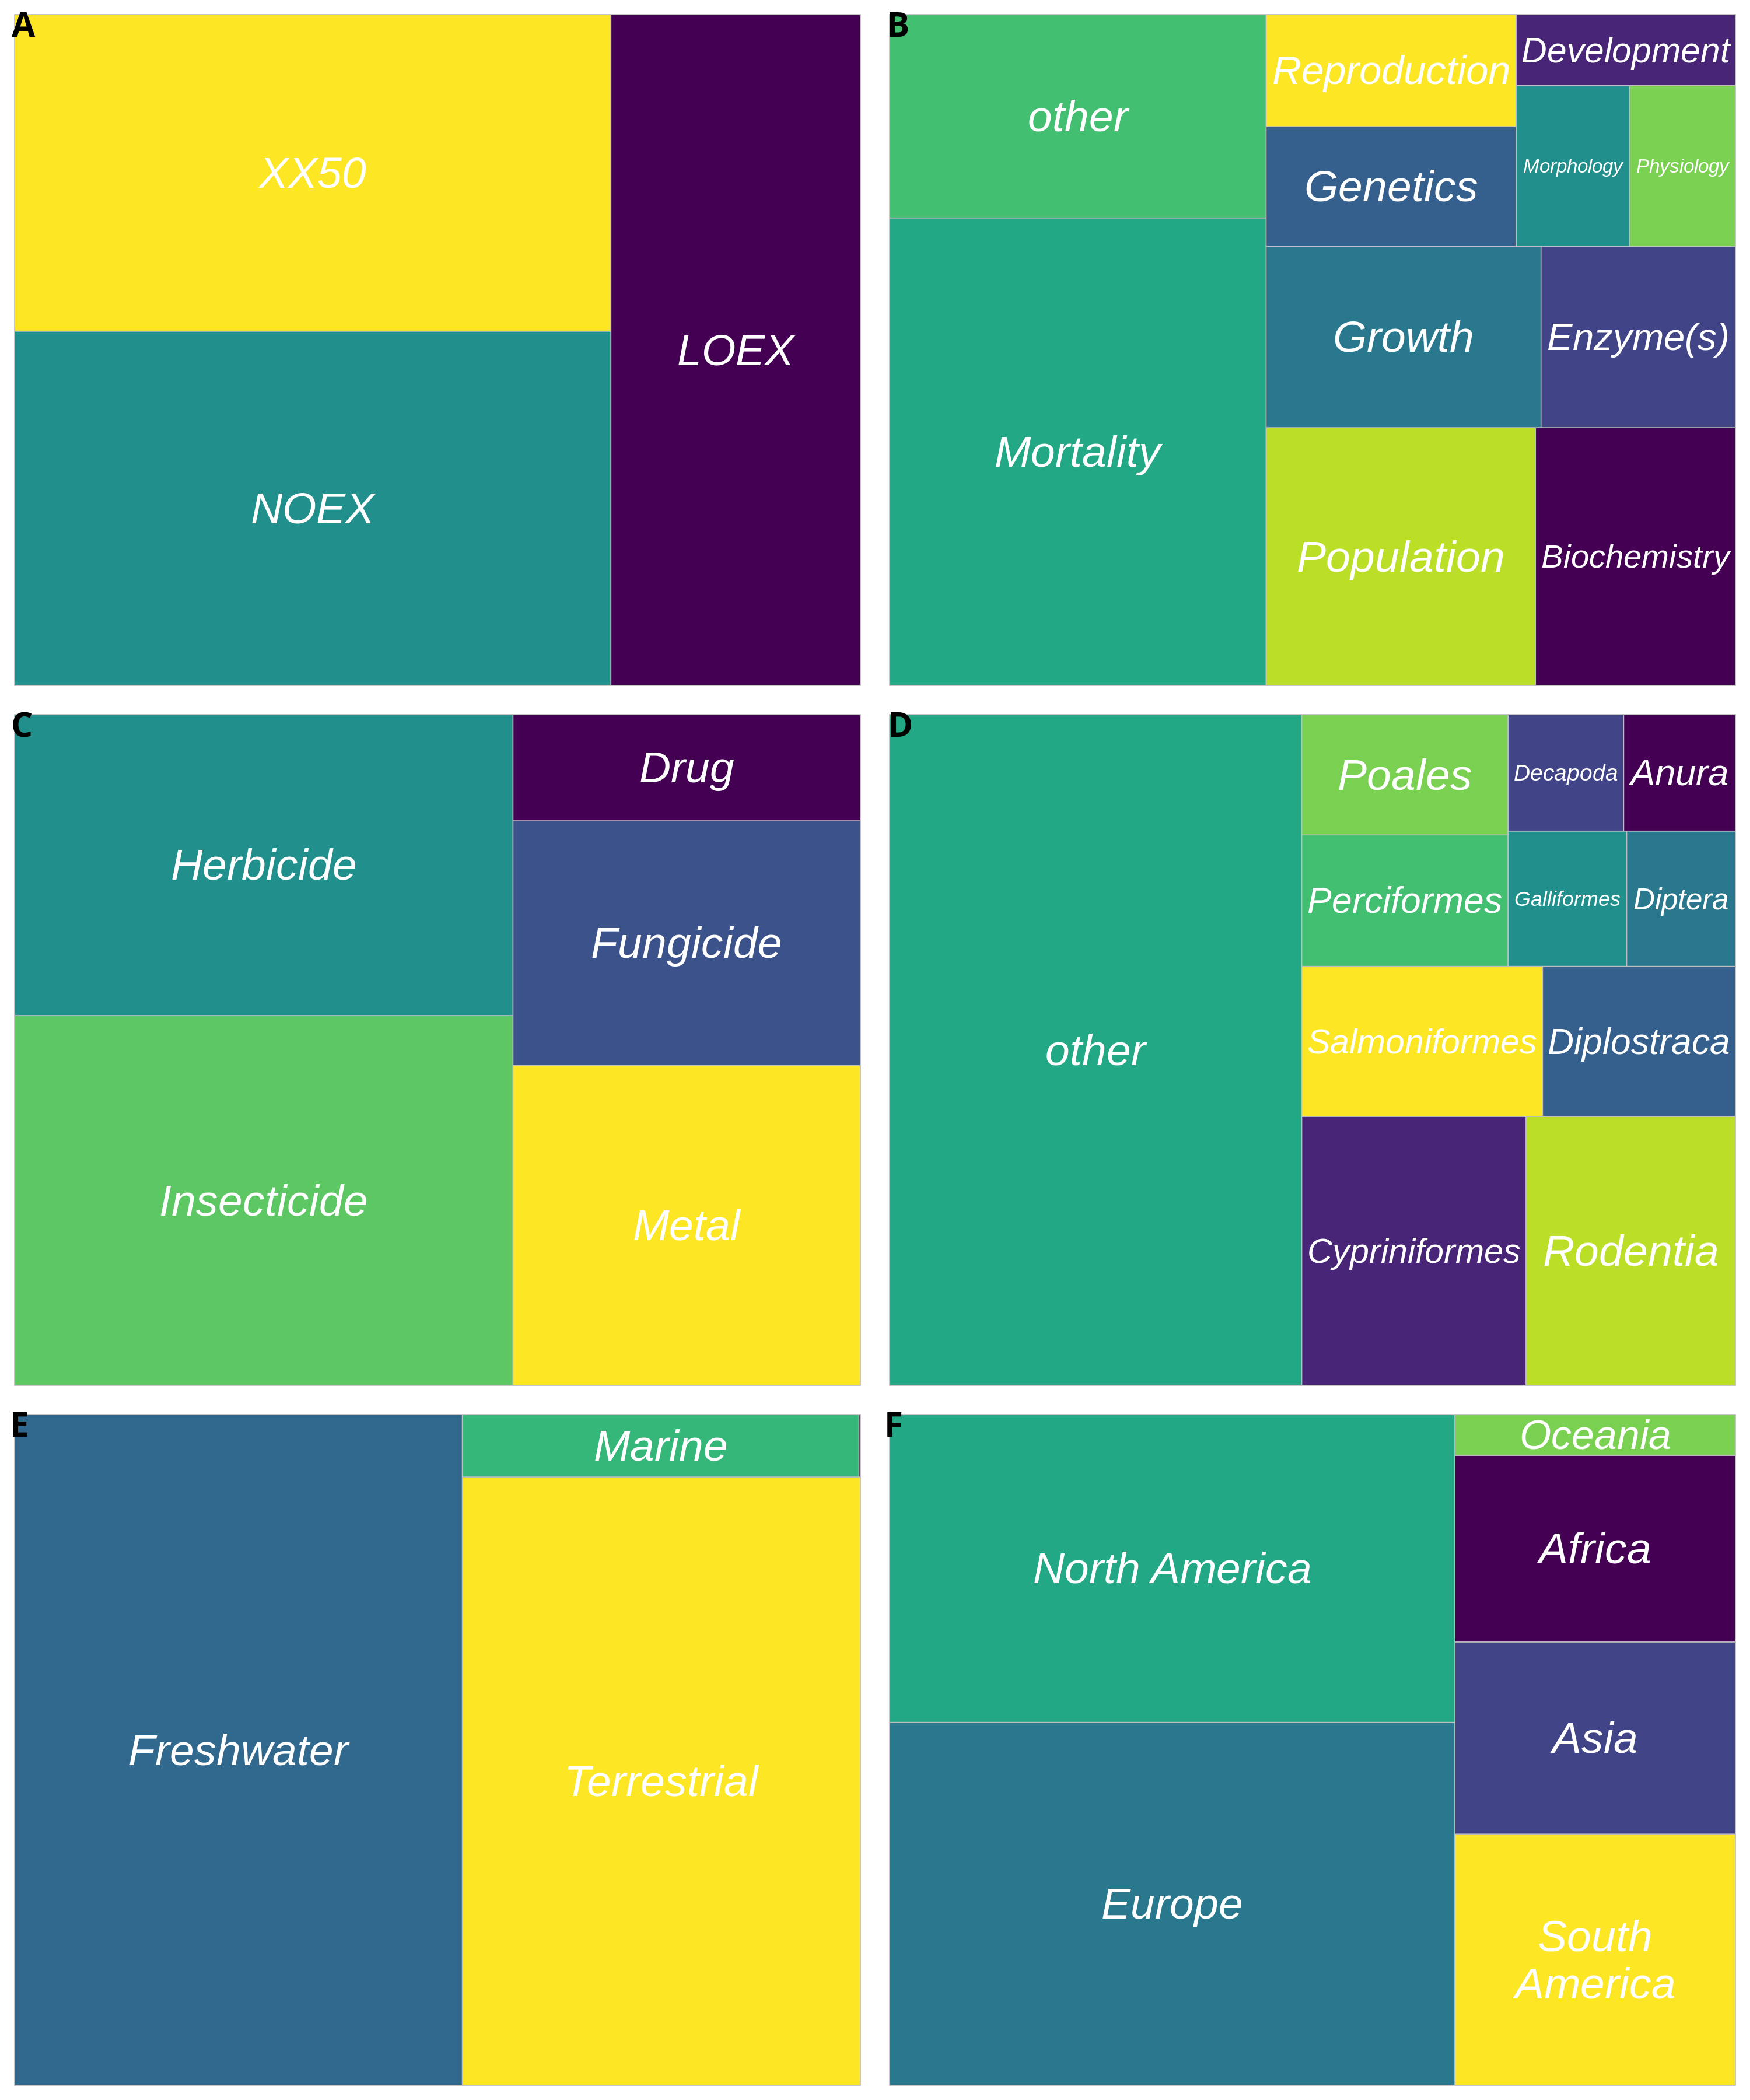
\includegraphics[width=1.0\textwidth]{article/figures/standartox_parameters.png}
    \caption{Share of 10 most frequent entries for the parameters effect group (A), chemical role (B), chemical class (C), taxonomic order (D), organism habitat (E) and organism occurrence region (F) in Standartox.}
    \label{fig:stx-parameters}
\end{figure}

\subsection{Aggregation}
Typically, species exhibit a differential sensitivity towards chemicals (Fig. \ref{fig:stx-variability}A). Moreover, multiple ecotoxicity values are available for individual species-chemical combinations and these can exhibit high variability due to several factors such as durations of ecotoxicity tests (Fig. \ref{fig:stx-variability}B), experimental conditions and physiology and genetic strain of the test individuals or populations. To aggregate multiple ecotoxicity values into a single value on the desired taxonomic level (e.g. for an individual species, across species of a genus or family), and chemical grouping (e.g. across all pesticides), Standartox provides several aggregation methods including the minimum, the maximum and the geometric mean as aggregates from the filtered data set for each chemical. The geometric mean is preferred in comparison to the arithmetic mean, because it is considerably less influenced by outliers and is suitable for skewed data. Also, the geometric mean is preferable over the median, because the median completely ignores the influence of large or small values, making it unreliable for small data sets. In the course of the aggregation process, outliers that exceed 1.5 times the interquartile range are flagged to caution Standartox users. However, since the geometric mean is relatively robust against outliers, they are not removed automatically. Overall, aggregation with Standartox allows to reduce the between-study variability when toxicity data are aggregated.

\begin{figure}[h!]
    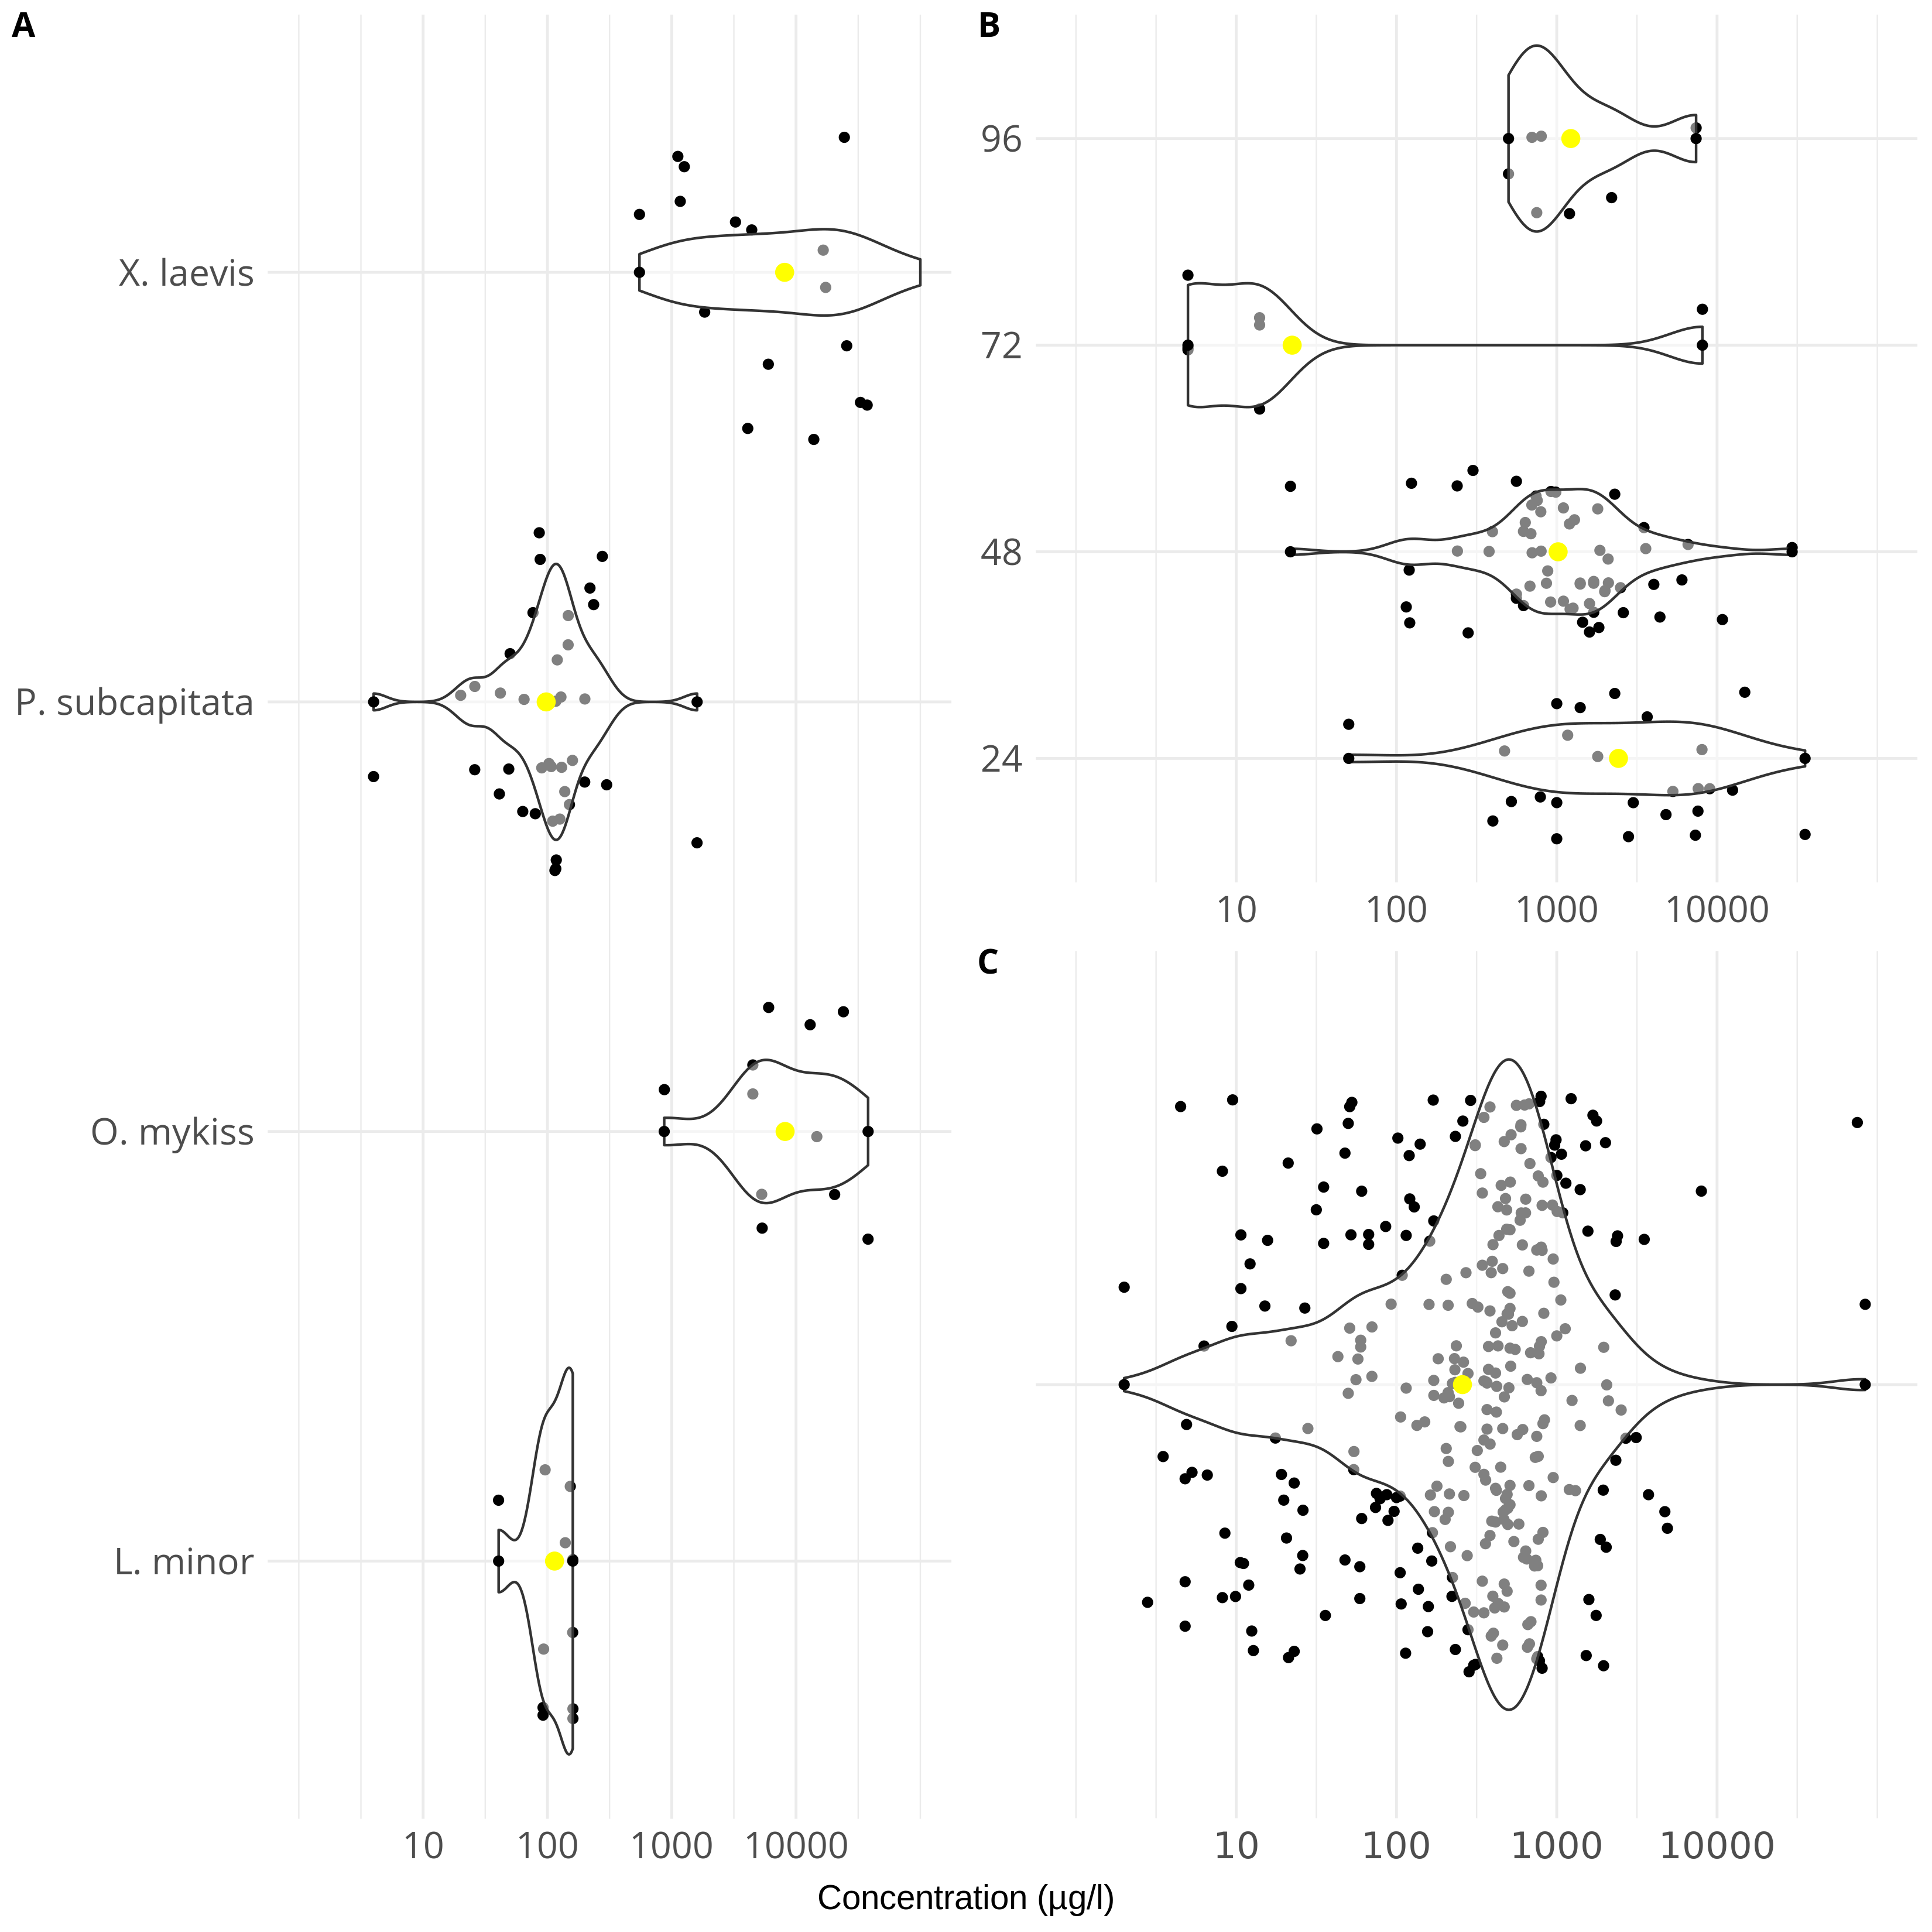
\includegraphics[width=1.0\textwidth]{article/figures/results_variability.png}
    \caption{Violin plots of the variability of test results (EC\textsubscript{50}) in Standartox because of different species (i.e. \textit{Xenopus laevis} - Amphibia, \textit{Raphidocelis subcapitata} - Algae, \textit{Oncorhynchus mykiss} - fish, \textit{Lemna minor} - invertebrate) to the chemical atrazine tested for 96 h (A), different durations of toxicity tests with zinc sulfate and \textit{Daphnia magna} (B) and unaccountable variability of cupric sulfate tested on \textit{Pimephales promelas} for 96 h (C). Purple dots depict Standartox geometric mean estimates and black dots show un-aggregated values for each group. To facilitate readability, data points are randomly scattered along a hypothetical y-axis and are greyed out within the violins.}
    \label{fig:stx-variability}
\end{figure}

\subsection{Accuracy Assessment}
To validate Standartox results we compared the aggregated results using the geometric mean to values from other databases. The PPDB provides ecotoxicity data on a few selected species from chemical risk assessment that have been manually quality controlled through expert judgement \citep{lewis_international_2016}. The vast majority of aggregated values (91 \%) of Standartox lie within one order of magnitude of the corresponding PPDB values (n = 3601). This would increase to 92.7 \%, when restricting the comparison to Standartox values where data from at least five experiments were available. Similarly, we compared Standartox to ecotoxicity values for \textit{D. magna} from the ChemProp \citep{ufzdepartmentofecologicalchemistry_chemprop_2019} software, which estimates LC\textsubscript{50} values via quantitative structure-activity relationship (QSAR) models \citep{schuurmann_quantitative_2011} We found that  95 \% of Standartox values lie within one order of magnitude of Chemprop (n = 179). However, the difference is not necessarily an indication of lower quality of Standartox estimates but may also reflect the wider range of experimental conditions for which data are available in the database underlying Standartox as well as inaccurate predictions for QSAR models, respectively (Figure \ref{fig:standartox_ppdb_diff}).

\begin{figure}[h!]
    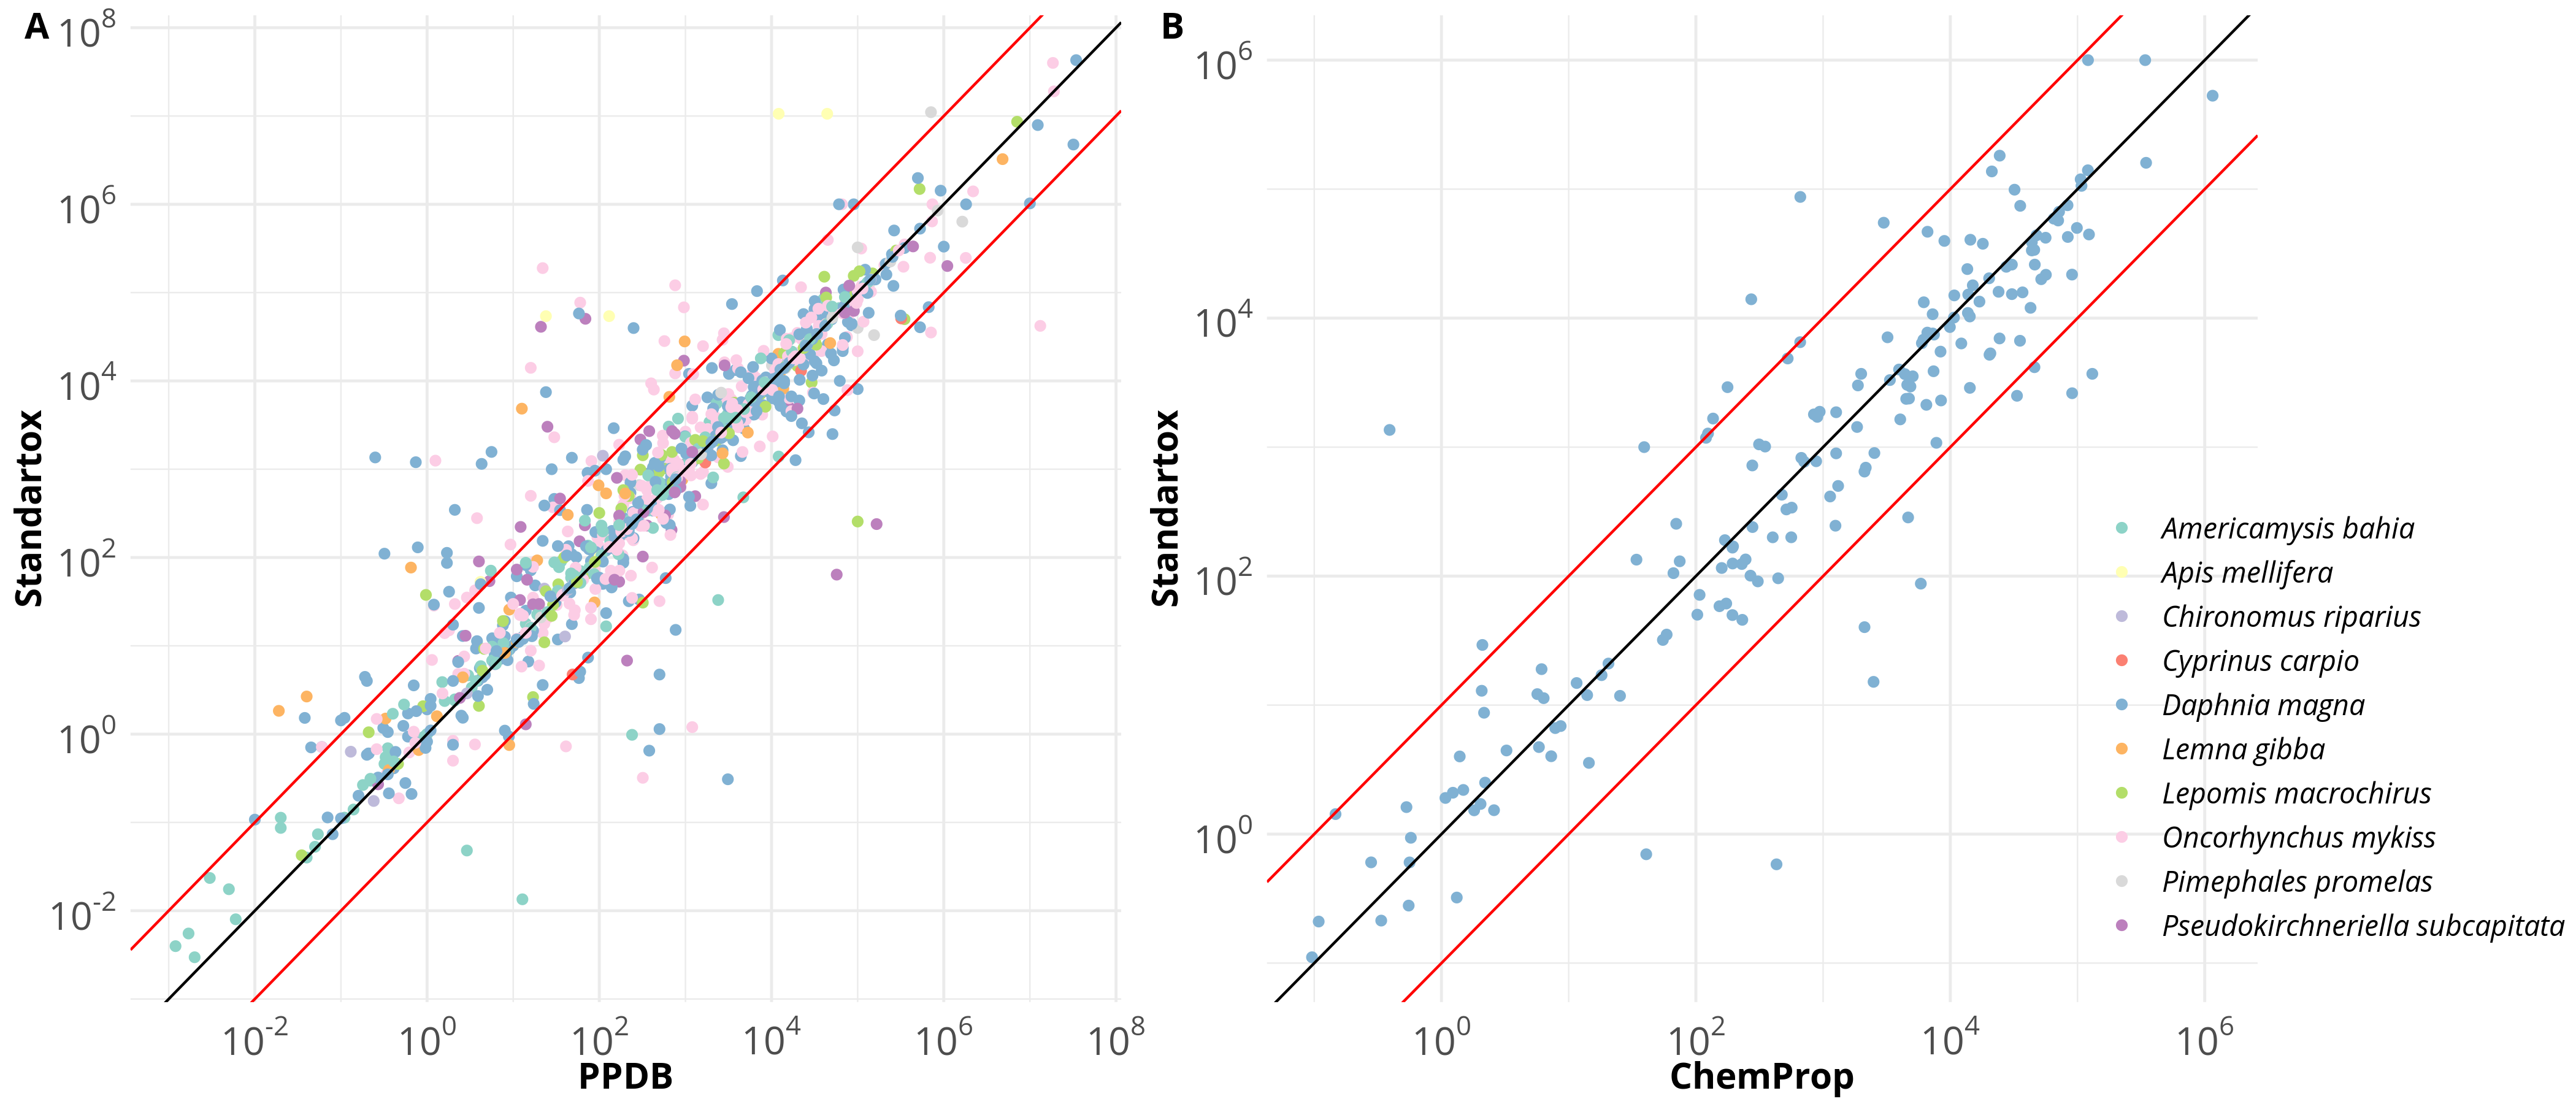
\includegraphics[width=1\linewidth]{article/figures/gg_ppdb_stan_compare_continous.png}
    \caption{Comparison between Standartox and (A) PPDB and (B) ChemProp values. The black lines indicate identity and red lines mark a divergence of a factor of 10. Compared species are color coded.}
    \label{fig:standartox_ppdb_diff}
\end{figure}

\subsection{Perspectives}
Novel predictive frameworks incorporating chemical mode of action and species traits emphasize the need for holistic and automated analyses of large-scale ecotoxicological data \citep{malaj_evolutionary_2016, vandenberg_modeling_2019}. Indeed, the increasing amount of data from ecotoxicological tests and experiments that is becoming available has elicited several initiatives to  harmonize these data. These initiatives partly aim for overlapping goals, yet have limitations or objectives that discriminate them from Standartox. The Network of reference laboratories, research centres and related organisations for monitoring of emerging environmental substances (NORMAN) focuses on assembling river basin specific pollutants from studies and databases \citep{von_der_ohe_new_2011}. The EnviroTox database \href{https://envirotoxdatabase.org/} which also uses, amongst others the ECOTOX database as an input has recently been published \citep{healthandenvironmentalsciencesinstitutehesi_envirotox_2019, connors_creation_2019}. In contrast to Standartox, EnviroTox  is restricted to selected aquatic organisms (i.e. fish, amphibians, invertebrates and algae) and experimental durations (at least 24 h) and uses a qualitative algorithm to derive single ecotoxicity values. Besides, EnviroTox provide additional information on toxicity endpoints, such as acute or chronic classifications and mode of action assignments. An action that can also be allocated to the user, since there are several different ways to classify such parameters, especially those mentioned, guaranteeing user flexibility. The EnviroTox database allows for an aggregation into single toxicity values for individual taxa,  whereas Standartox performs this aggregation for individual taxa-chemical combinations. However, the Standartox results for individual taxa-chemical combinations could easily be aggregated across chemicals in a second step based on chemical parameters. Comptox, is a web tool published by the EPA which, similar to Standartox allows for filtering test results, the retrieval of additional chemical information and predicting toxicity properties, such as 48 h \textit{Daphnia magna} LC\textsubscript{50} values. However, toxicity predictions are limited to standard organisms (e.g. \textit{Daphnia magna}), and the tool lacks the possibility for automatic retrieval of predicted \citep{williams_comptox_2017}. 


In summary, none of the above mentioned initiatives aim for a holistic and automated standardized aggregation method of exposure endpoints for individual chemicals. In addition, they lack the possibility to access the databases through common high level programming languages, such as R. As outlined above, toxicity estimates from different studies can be highly variable due to a wide range of experimental conditions such as pH, temperature or conductivity \citep{rosenkrantz_influence_2013, li_temperature_2011}. Integrating these factors into the aggregated estimates would improve toxicity estimates . However, the current implementation of Standartox does not consider these factors, because the ECOTOX database only provides sparse records on experimental conditions. The most frequently provided experimental conditions are temperature (77 \%), pH (56 \%), hardness (27 \%), dissolved oxygen (18 \%), Alkalinity (15 \%) and salinity (9 \%), and all others for less than 5 \%. A text-mining approach, where a literature reference is associated with  ecotoxicity raw data, iterating through the individual publications could potentially increase this number.

%% table that compares different ecotoxicological databases

%%%% CONTINUE HERE

\begin{sidewaystable}
% \begin{table}
\caption{Different databases that provide ecotoxicological data. Abbreviations: \textbf{ALL:} Most important test parameters, including chemical, taxon, duration for filtering ecotoxicological data are incorporated. \textbf{WEB:} Accessible via a web application through a graphical user interface. \textbf{API:} Accessible via an application programming interface.}
\label{tab:database-differences}
\begin{tabular}{|m{3cm}|m{3cm}|m{2cm}|m{2cm}|m{1cm}|l|}
\hline
Database & Publisher & Filter & Aggregation, Selection & Access & website \\
\hline
Comptox & Environmental Protection Agency & Chemical & no & WEB, file & https://comptox.epa.gov/dashboard \\
\hline
Ecotox & Environmental Protection Agency & ALL & no & WEB, file & https://webetox.uba.de/webETOX/index.do \\
\hline
EnviroTox & Health and Environmental Sciences Institute & ALL & chemical, organism & WEB & https://envirotoxdatabase.org \\
\hline
Etox & Umweltbundesamt & ALL & no & WEB & https://webetox.uba.de/webETOX/index.do \\
\hline
Pesticide Property Data Base (PPDB) & University of Hertfordshire & fixed values & manual selection & WEB, file & https://sitem.herts.ac.uk/aeru/ppdb/index.htm \\
\hline
\textbf{Standartox} & \textbf{this article} & \textbf{ALL} & \textbf{chemical, organism} & \textbf{API, WEB} & \textbf{http://standartox.uni-landau.de} \\
\hline
\end{tabular}
% \end{table}
\end{sidewaystable}










